\documentclass[0-thesis.tex]{subfiles}
\begin{document}
The previous sections proposed the update architecture of the thesis, its key components,
and security considerations such as identity and access control. Two profiles
instantiating the architecture were also presented. This section discusses a prototype
implementation of the architecture as well as a manifest generator. 

\subsection{Manifest Implementation}
\label{ssec:manifest-implementation}
As manifests contain certain information difficult for humans to provide such as
monotonically increasing sequence numbers and hash digests, a manifest generator was
created to help test the prototype \parencite{manifest-generator}. It is a Python script
which accepts information about vendor and class namespace, version, image file, and
associated URL in order to generate and format a manifest both in JSON and CBOR. The
outputted manifest follows the format specified in Section~\ref{ssec:manifest-format} and
features all required fields although some left blank. It is a bare-bones manifest
containing only the required information for a singular, monolithic update. There are no
dependencies or options specified.

The manifest is a JSON map featuring the required elements shown in
Figure~\ref{fig:manifest-format}. The elements are in the same order as in the figure but
the names of the fields have been substituted for integers in order to save space.
Table~\ref{tab:manifest-substitution} shows this mapping. Repeatable structures such as
preconditions are described as a nested array of maps, where each map in the array
constitutes one instance of such an element. The keys in these nested maps are also mapped
to integers as in the main manifest structure, but resetting the counter for each map. The
mapping of keys in nested structures is shown in Table~\ref{tab:nested-substitution}. The
example manifest used in the thesis is found in Appendix~\ref{app:manifest}. 

\begin{longtable}[]{@{}ll@{}}
    \caption{Mapping manifest elements to integers as keys in the JSON manifest.}
    \label{tab:manifest-substitution}\\
    \toprule
    Element Name & Mapped To\tabularnewline
    \midrule
    \endhead
    versionID & 0\tabularnewline
    sequenceNumber & 1\tabularnewline
    preConditions & 2\tabularnewline
    postConditions & 3\tabularnewline
    contentKeyMethod & 4\tabularnewline
    payloadInfo & 5\tabularnewline
    precursorImage & 6\tabularnewline
    dependencies & 7\tabularnewline
    options & 8\tabularnewline
    \bottomrule
\end{longtable}

\newpage    % To avoid splitting the relatively short table
\begin{longtable}[]{@{}ll@{}}
    \caption{Mapping elements in nested structures to integers.}
    \label{tab:nested-substitution}\\
    \toprule
    Element Name (corresponding structure) & Mapped To\tabularnewline
    \midrule
    \endhead
    type (conditions and options) & 0\tabularnewline
    value (conditions and options) & 1\tabularnewline
    \bottomrule
    URL (URL/digest pair) & 0\tabularnewline
    digest (URL/digest pair) & 1\tabularnewline
    \bottomrule
    format (payload info) & 0\tabularnewline
    size (payload info) & 1\tabularnewline
    storage (payload info) & 2\tabularnewline
    URL/digest pair (payload info) & 3\tabularnewline
    \bottomrule
\end{longtable}

In the client code, the manifest is received as a string, still formatted as JSON. In
order to parse it, structs resembling the format of the manifest were created, see
Listing~\ref{lst:manifest}. The base manifest structure contains values of version ID,
sequence number, and content key method alongside pointers to other parts of the manifest.
These parts, represented as repeated maps in the JSON string, are implemented as linked
lists in order to store an arbitrary amount of such structures. With the example manifest
shown in Appendix~\ref{app:manifest}, the base manifest structure would for instance
contain a two element long linked list of preconditions (vendor ID then class ID). Certain
manifest elements, namely precursor image, dependencies, and URL/digest pair in payload
info convey the same kind of information but are separated into different lists because of
the differences in semantics.

\begin{lstlisting}[language=manifest, caption={The client manifest implementation.}, label=lst:manifest]
    typedef struct manifest_s {
        uint8_t versionID;
        uint32_t sequenceNumber;
        struct condition_s *preConditions;
        struct condition_s *postConditions;
        uint8_t contentKeyMethod;
        struct payloadInfo_s *payloadInfo;
        struct URLDigest_s *precursorImage;
        struct URLDigest_s *dependencies;
        struct option_s *options;
    } manifest_t;

    typedef struct condition_s {
        int8_t type;
        char *value;
        struct condition_s *next;
    } condition_t;

    typedef struct payloadInfo_s {
        uint8_t format;
        uint32_t size;
        uint8_t storage;
        struct URLDigest_s *URLDigest;
    } payloadInfo_t;

    typedef struct URLDigest_s {
        char *URL;
        char *digest;
        struct URLDigest_s *next;
    } URLDigest_t;

    typedef struct option_s {
        int8_t type;
        char *value;
        struct option_s *next;
    } option_t;
\end{lstlisting}


\subsection{Prototype Implementation}
\label{ssec:prototype-implementation}
The prototype used in the thesis was developed in order to measure the efficiency of
transport during an update procedure as well as serving as a source of inspiration for
other implementers. It consists of a server and a client both implemented in Contiki-NG,
thus written purely in C. The server was implemented in Contiki-NG as a proof-of-concept
that a more capable IoT device could be used as an update server. The prototype uses a
pull model meaning the client initiates the update procedure and the server responds with
a corresponding resource. All traffic is sent via CoAPs encrypted by DTLS. Certificate
support in Contiki-NG was at the time of implementation missing, thus pre-shared keys for
DTLS were used instead. Figure~\ref{fig:client-server-interaction} shows the interactions
between the client and server.

\begin{figure}[h!]
    \caption{The interactions of client and server during an update procedure.}
    \label{fig:client-server-interaction}
    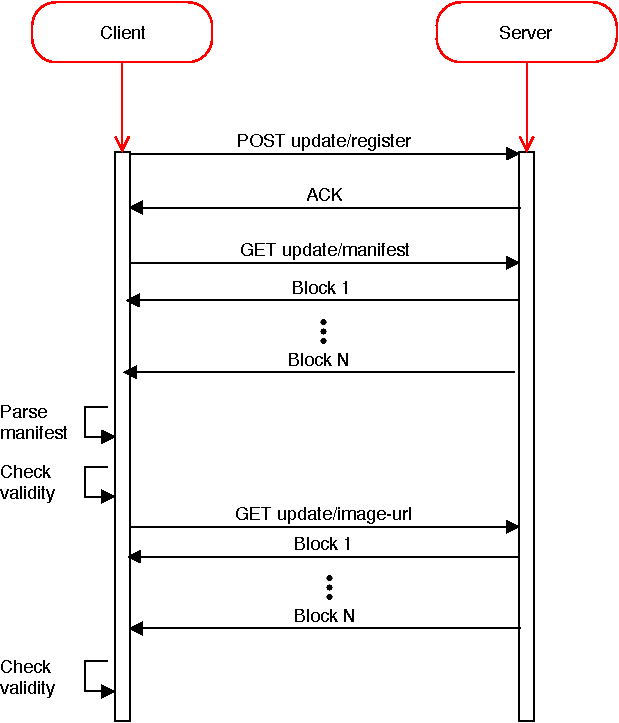
\includegraphics{images/client-server-sequence.pdf}
\end{figure}

The server implements three resources mapped to the endpoints \texttt{update/register},
\texttt{update/manifest}, and \texttt{update/image}. The register resource listens to POST
requests and upon a request extracts the vendor ID, class ID, and version number sent by
the client and creates a profile file before answering with message code 2.01 CREATED.
Other information can be put into the profile, such as choice of protocol and IP address,
in order to reach the device again. For the prototype, such information was not needed,
and the file was created just as proof-of-concept.

In a real deployment with different devices, thus different manifests, the manifest
resource is responsible for picking a suitable manifest based on the information in the
device's profile. For the prototype only one manifest was used which was hard-coded into
the manifest resource. Upon a GET request to the manifest resource the manifest is
encrypted through COSE and sent using CoAP's block option. The entire manifest is
encrypted at once and the ciphertext sent block by block. Since the manifest is
relatively small it is easy to allocate buffers large enough to encrypt the entire
manifest at once, leading to smaller overhead. Ideally the manifest would be signed with
COSE instead of encrypted. COSE implementations in Contiki-NG were limited and at the time
of development signing was not available and implementing it would prove too time
consuming. Encrypting the manifest requires a bit more information than signing, such as a
nonce and Additional Authenticated Data. These were hard coded in both client and server,
alongside the key.

Lastly, the image resource generates data in a deterministic manner, COSE encrypts it
block by block, and sends through CoAP's block option. Ideally this data would also be
signed instead of encrypted. The reasoning for encrypting the data block by block is that
should a large amount of data be sent, such as a firmware image, it would be difficult to
allocate buffers large enough to process the entire image at once, both for the server and
client. Instead it is encrypted and decrypted blockwise. While this solves the issue of
encrypting and decrypting large amounts of data, it introduces a larger overhead as each
32 byte block sent will contain 24 bytes of data and 8 bytes of tag for validation. The
manifest resource only introduces this overhead once while the image resource introduces
it once per block.

The client performs three remote calls to the server, one call to each resource, and
performs some additional operations related to the manifest and image data. First a POST
request is sent to the update/register endpoint. The client does not need to act upon the
response. Afterwards a GET request is sent to the update/manifest endpoint. The manifest
callback buffers the manifest into memory block by block and when the callback finishes
decrypts the entire manifest at once. After decryption it is parsed into structs shown in
Listing~\ref{lst:manifest} and pre-conditions are checked. If any other fields that need
checking before proceeding, such as optional pre-directives, they would also be checked at
this point. 

If the client deems the manifest to be correct it uses the URL found in the
\texttt{payloadInfo->URLDigest} struct to call upon that URL. In this case it is
\texttt{update/image}, but could be any endpoint hosting a resource specific for that
class of device. The image callback decrypts and updates a SHA-256 context with the
plaintext blockwise. After the transfer concludes, the checksum of the image data is
calculated and compared to the one in the manifest.


\subsection{Summary}
\label{ssec:implementation-summary}
This chapter presented a DTLS/CoAPs prototype of the proposed architecture. The prototype
is made up of a client and a server developed in Contiki-NG as well as an instantiation of
the manifest format presented in Section~\ref{ssec:manifest-format}. The prototype is
based on the pull model, meaning it is client initiated, and goes through the steps of
registering, receiving a manifest, and receiving image data. It uses COSE encryption and
pre-shared DTLS keys as COSE signing and certificate support was at the time not available
in Contiki-NG. It also does not use tokens as it represents a monolithic update and not
differential update. The next chapter will evaluate the architecture in a qualitative
manner and the prototype in a quantitative manner in order to see if it fulfills the goals
of SUIT and contextualize the implementation.

\end{document}